
% The \phantomsection command is needed to create a link to a place in the document that is not a
% figure, equation, table, section, subsection, chapter, etc.
% https://tex.stackexchange.com/questions/44088/when-do-i-need-to-invoke-phantomsection
\phantomsection

% Multiple-language document - babel - selectlanguage vs begin/end{otherlanguage}
% https://tex.stackexchange.com/questions/36526/multiple-language-document-babel-selectlanguage-vs-begin-endotherlanguage
\begin{otherlanguage*}{brazil}

    \chapter{Trabalhos Relacionados}

    Neste capítulo primeiramente é apresentado um artigo que descreve um modelo de plano de ensino pautado na plataforma Beecrowd, bem como suas justificativas e aspectos positivos. Após isso, foram selecionados três artigos que mostram integração de diferentes ambientes de desenvolvimento com o Moodle: o BOCA, o CodeRunner, e o VPL.


\section{UTILIZAÇÃO DA PLATAFORMA BEECROWD DE MARATONA DE PROGRAMAÇÃO COMO ESTRATÉGIA PARA O ENSINO DE ALGORITMOS}

Neste estudo conduzido por \cite{cruz2022}, é apresentada uma proposta de plano de ensino que se baseia no aproveitamento da plataforma Beecrowd para maratonas de programação, alinhada a abordagens pedagógicas ativas. Dessa maneira, são integrados conceitos como sala de aula invertida e gamificação, proporcionando uma abordagem dinâmica e envolvente no processo de aprendizagem e explorando as potencialidades da plataforma Beecrowd para oferecer uma experiência educacional inovadora. 

Os autores têm como objetivo aplicar essa metodologia de maneira a diminuir a curva de aprendizagem dos alunos, apoiar os professores na implementação de abordagens pedagógicas ativas em sala de aula e ampliar as oportunidades de interação entre os alunos, contribuindo assim para o desenvolvimento do aprendizado.

Os autores destacam a gamificação e a sala de aula invertida como estratégias que integram métodos de ensino com diversos recursos de comunicação, incluindo materiais escritos, orais e audiovisuais, junto a atividades, desafios e informações contextualizadas. A gamificação é apresentada como a aplicação de elementos característicos de jogos, uma abordagem eficaz para transformar a forma como os estímulos são apresentados aos alunos, visando engajá-los e incentivá-los a resolver problemas da maneira mais eficiente possível. 

De maneira semelhante, a sala de aula invertida é descrita como uma proposta para dinamizar a transmissão de informações durante as aulas, utilizando ferramentas online estruturadas e bem planejadas. Essa abordagem visa incentivar a iniciativa dos alunos ao estudarem previamente determinados conteúdos antes das aulas ministradas pelos professores.

Os autores ressaltaram a importância da disciplina de algoritmos como a base fundamental para o ensino de programação em diversos cursos na área da Informática. Essa disciplina aborda princípios essenciais de lógica de programação, visando desenvolver a capacidade dos estudantes em analisar e resolver problemas por meio da criação de algoritmos. Contudo, enfrenta desafios significativos, evidenciados pelo elevado índice de evasão e reprovação, tornando-se um ponto crítico nos cursos de graduação e impactando a continuidade dos alunos. 

A complexidade reside, em grande parte, na diversidade de alunos e em seus distintos estilos e ritmos de aprendizado, conforme indicado pelos autores. A adaptação eficiente a essa heterogeneidade representa um desafio no ensino de algoritmos e programação para novos estudantes. Nesse contexto, os autores propõem que a utilização de ferramentas online amplamente disponíveis para a aprendizagem ativa pode ser uma estratégia eficaz para permitir que cada aluno progrida em seu próprio ritmo e velocidade \cite[p.~5]{cruz2022}. 

No que diz respeito à integração de questões de maratonas de programação em sala de aula, os autores destacam sua relevância ao promover a busca ativa pela resolução de problemas. Ao buscar soluções, os alunos não apenas adquirem conhecimento sobre tópicos ainda não abordados em aula, mas também consolidam conceitos previamente ensinados.

O Beecrowd se destaca como uma ferramenta online que não apenas viabiliza a resolução de problemas em competições de programação, mas também se apresenta como uma valiosa aliada para o trabalho do professor. Os autores do estudo evidenciam que os desafios oferecidos pela plataforma Beecrowd estão meticulosamente organizados em categorias e níveis de dificuldade. As categorias abrangem temas como Iniciante, AD-HOC, Strings, Estruturas e Bibliotecas, Matemática, Paradigmas, Grafos, Geometria Computacional e SQL. A escala de dificuldade varia de 1 a 10, sendo 1 as questões mais acessíveis e 10 as mais desafiadoras.

No âmbito do artigo analisado, foram selecionadas questões da categoria Iniciante, e a partir delas, elaborou-se um plano de ensino voltado para a implementação da metodologia ativa da maratona de programação. Este plano foi aplicado em seis semestres na disciplina de algoritmos, envolvendo alunos que, em sua maioria, não possuíam conhecimento prévio em programação. A avaliação da proposta foi conduzida ao longo de três semestres que adotaram as metodologias ativas e outros três semestres que não as utilizaram, de forma intercalada. 

Através desse experimento e da análise de seus resultados, os autores constataram que a aplicação das metodologias de gamificação e sala de aula invertida contribuiu significativamente para o desempenho da turma, observando-se um crescimento notável. Além disso, as notas mais elevadas foram mais consistentes ao longo do tempo, demonstrando a eficácia dessas abordagens no contexto educacional.

Dessa forma, constatou-se que integrar o Beecrowd como um suporte para a implementação da gamificação como metodologia ativa na disciplina de algoritmos foi eficaz. A adoção do formato de maratona de programação possibilita ao professor envolver os alunos de forma mais imersiva, enquanto a plataforma oferece suporte adicional para o desenvolvimento da disciplina. Isso não apenas aprimora o processo de ensino e aprendizagem, mas também contribui para a redução da evasão em cursos superiores de informática.



\section{INTEGRAÇÃO DO AMBIENTE BOCA COM O AMBIENTE MOODLE PARA AVALIAÇÃO AUTOMÁTICA DE ALGORITMOS}

No estudo conduzido por \cite{galasso}, destaca-se a integração entre o BOCA Online Contest Administrator e a plataforma Moodle, focalizando a disciplina de algoritmos como um pilar crucial no ensino da programação. O estudo ressalta a importância de proporcionar uma experiência facilitada tanto para alunos quanto para professores, reconhecendo-a como essencial para o eficaz aprendizado e aproveitamento dessa disciplina. 

O BOCA Online Contest Administrator representa um ambiente dedicado à administração de competições que abrangem a programação de computadores, incluindo eventos como a Maratona de Programação. Uma característica fundamental é a presença de um juiz online que realiza avaliações automáticas dos algoritmos submetidos pelos participantes. 

Os autores do estudo concentraram seus esforços no desenvolvimento dessa integração, visando possibilitar a criação de questões na plataforma Moodle nas quais as respostas consistem de algoritmos. Estes, por sua vez, são avaliados de forma automática, gerando resultados para cada submissão dos alunos. Além disso, a integração foi concebida de modo a garantir que os ambientes envolvidos fossem implementados em servidores independentes. Isso assegura que a utilização do BOCA durante a avaliação dos algoritmos não comprometa o desempenho do ambiente Moodle.

Dessa forma, a proposta apresentada introduz um novo tipo de questão, denominada "Juiz online", destinada a ser incorporada nos questionários do ambiente Moodle. O processo requer que o professor insira uma questão para cada problema que deseja abordar. Uma vantagem oferecida pelo próprio Moodle é a capacidade do professor de utilizar várias dessas questões para compor um questionário abrangente.
	
Para construir os problemas, o professor preenche campos específicos no ambiente Moodle, incluindo o título do problema, o corpo do problema (enunciado) e um conjunto de casos de teste. Cada caso de teste inclui entradas para o algoritmo e a saída esperada correspondente à entrada fornecida. Durante o cadastro, é necessário especificar a linguagem de programação para a resolução do problema. A instalação padrão do BOCA suporta as linguagens C, C++ e Java, compilando o algoritmo com o compilador apropriado para a linguagem indicada no momento do cadastro.

Os alunos submetem algoritmos em código-fonte no Moodle, utilizando a linguagem indicada pelo professor. Depois, o BOCA avalia automaticamente, compilando e executando o código com entradas cadastradas pelo professor, e comparando com uma saída padrão predefinida. A resposta ao aluno pode ser apenas correta ou incorreta, sem possibilidade de avaliação parcial. Diversos tipos de erros podem ocorrer, tais como problemas de compilação, formatação inadequada ou tempo excedido. O Moodle permite múltiplas tentativas, proporcionando aos alunos a oportunidade de corrigir possíveis equívocos. Além disso, o professor tem a prerrogativa de ajustar manualmente os resultados, focando sua avaliação nas partes incorretas, o que contribui significativamente para aliviar a carga de correções.
 
A figura 10 representa uma edição da tela de cadastro da questão, proporcionando uma visão ilustrativa desta fase do processo, já a figura 11 oferece uma representação visual da avaliação de uma questão como correta.

\begin{figure}[h!]
	   \centering
            \caption{Integração BOCA-Moodle - Edição de tela de cadastro de questão}
            \label{fig:ModeloConceitual}
	   	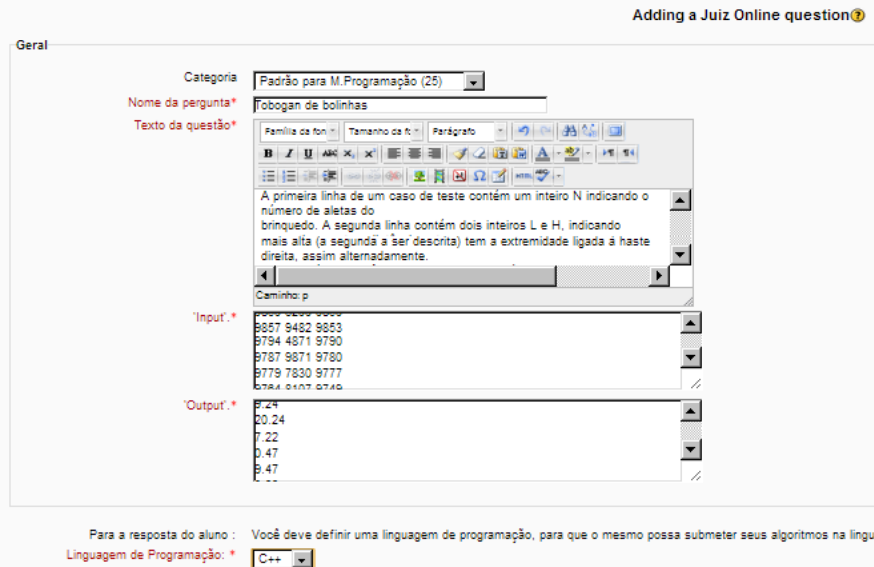
\includegraphics[scale=0.3]{pictures/BOCA_edicao.png}
        \fonte{\cite[p.~26]{galasso}}
\end{figure}

\begin{figure}[h!]
	   \centering
            \caption{Integração BOCA-Moodle - Visualização do retorno da avaliação da questão}
            \label{fig:ModeloConceitual}
	   	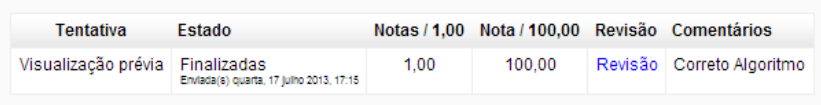
\includegraphics[scale=0.3]{pictures/BOCA_visualizacao.png}
        \fonte{\cite[p.~27]{galasso}}
\end{figure}

Nesta solução, é recomendável que o Moodle e o BOCA sejam executados em servidores separados. Essa abordagem visa garantir que uma possível sobrecarga no BOCA, ao avaliar muitos algoritmos, não comprometa o desempenho do Moodle. É importante observar que o BOCA foi desenvolvido para o Sistema Gerenciador de Banco de Dados (SGBD) PostgreSQL, exigindo que o Moodle seja instalado utilizando o mesmo sistema \cite[p.~27-28]{galasso}. 

Para possibilitar a comunicação entre bancos de dados em locais distintos, os autores usaram o Dblink no PostgreSQL. Segundo eles, Dblink, um conjunto de funções, facilita a conexão entre bancos de dados PostgreSQL para acesso a dados externos. Essa funcionalidade permite o acesso remoto a tabelas específicas em uma base de dados, bem como a execução de consultas \cite[p.~27-28]{galasso}.

Os autores destacaram também que o banco de dados do sistema BOCA consiste em doze tabelas, sendo quatro delas essenciais para o funcionamento do juiz online do BOCA: Problemtable, utilizada para cadastro de questões na competição; Runtable, usada quando o aluno submete algoritmos; Answertable, armazenando dados de correção após o algoritmo ser executado; e Langtable, a qual armazena as linguagens de programação a serem utilizadas. Além disso, duas tabelas adicionais, "tempaluno" e "tempprofessor", foram criadas para a manipulação de dados entre as tabelas preexistentes \cite[p.~27-28]{galasso}. 

“A integração do BOCA com o ambiente Moodle foi realizada através da criação de gatilhos (triggers), que é um recurso existente em diversos SGBD, dispensando alterações no código do Moodle e do BOCA” \cite[p.~28-29]{galasso}. A Figura 12 oferece uma visualização do fluxo de dados entre as bases de dados, destacando a atuação dos gatilhos.

\begin{figure}[h!]
	   \centering
            \caption{Integração BOCA-Moodle - Fluxo da interação das bases de dados do Moodle e do BOCA}
            \label{fig:ModeloConceitual}
	   	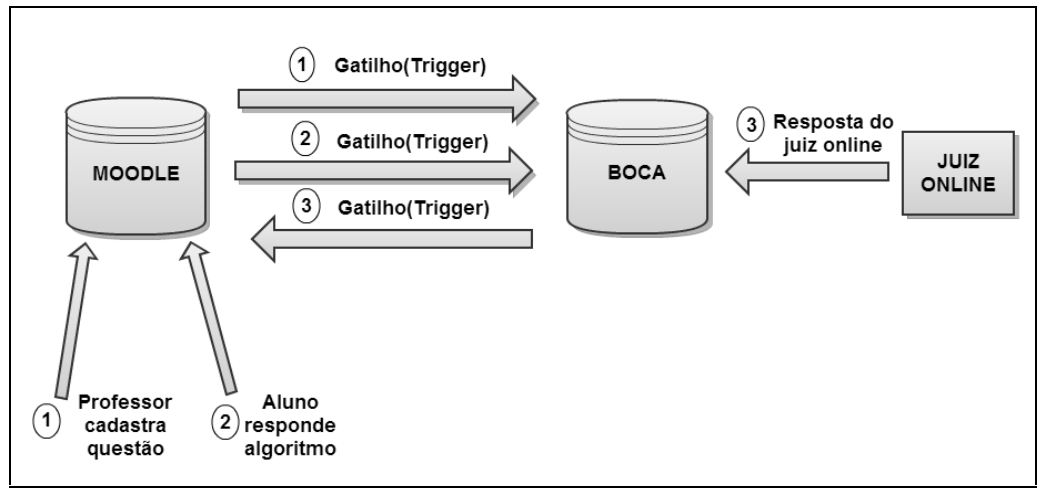
\includegraphics[scale=0.3]{pictures/BOCA_fluxo.png}
        \fonte{\cite[p.~29]{galasso}}
\end{figure}

Os autores explicaram o fluxo de gatilhos exibidos na figura 12:


\begin{enumerate} [label=(\alph*)]
    \item Quando um professor cadastra uma questão no Moodle, essa informação é registrada no banco de dados do Moodle, ativando o primeiro gatilho;
    \item Este gatilho grava os dados da questão na tabela "tempprofessor" no banco de dados do BOCA;
    \item Uma vez que os dados são registrados na tabela "tempprofessor", outro gatilho é acionado, carregando os dados relacionados ao problema criado pelo professor, incluindo o arquivo compactado com as configurações da questão necessário para o BOCA;
    \item Esses dados são então adicionados à tabela "problemtable", registrando assim o problema no BOCA;
    \item À medida que os alunos respondem às questões no Moodle, os envios são registrados nas tabelas do banco de dados do ambiente e um novo gatilho é acionado para a tabela "tempaluno";
    \item Posteriormente, outro gatilho registrado no BOCA entra em ação, pegando o arquivo com a resposta do aluno e as informações da questão, cadastrando-os na tabela "runtable" do BOCA.
\end{enumerate}

O BOCA utiliza um processo chamado "autojuding\" para verificar a correção de problemas submetidos. Esse script PHP, em execução contínua no servidor, compila o algoritmo do aluno, comparando a saída com a padrão definida pelo professor. A avaliação ocorre a cada minuto, identificando e julgando novos problemas. Os resultados são registrados na tabela "runtable" do BOCA, acionando um gatilho que atualiza as tabelas no Moodle para que os alunos visualizem o feedback  \cite[p.~29]{galasso}.

Ao submeter uma questão, é exibida uma imagem de carregamento indicando a espera pelo julgamento. Após a avaliação, a área do algoritmo muda para verde se a resposta estiver correta, ou vermelho para resposta incorreta. A figura 13 ilustra um exemplo  \cite[p.~30]{galasso}.

\begin{figure}[h!]
	   \centering
            \caption{Integração BOCA-Moodle - retorno da avaliação da questão como correta}
            \label{fig:ModeloConceitual}
	   	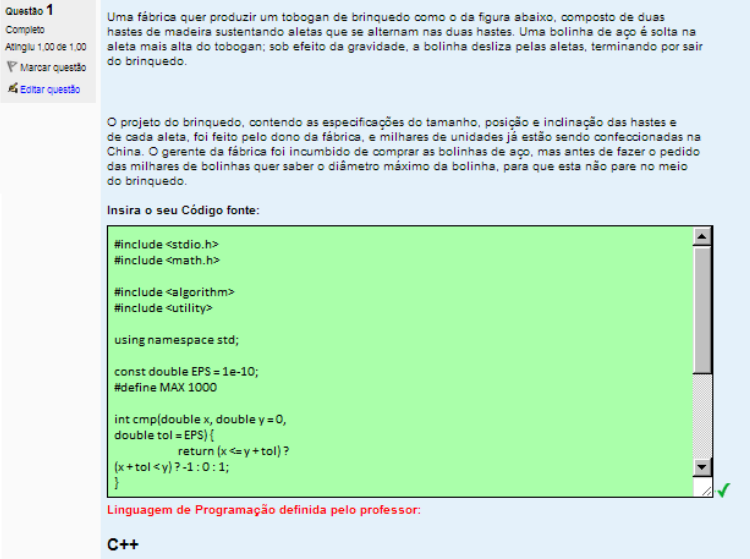
\includegraphics[scale=0.5]{pictures/BOCA_correta.png}
        \fonte{\cite[p.~26]{galasso}}
\end{figure}

Os autores revelaram que foi encontrado um erro ao fazer uma tentativa de enviar um arquivo “zip” diretamente para o banco de dados. Também não foi possível enviar arquivos de entrada e saída diretamente pelo banco de dados, resultando em problemas de codificação das tabulações e identificadores de nova linha. A solução envolveu o envio desses arquivos via FTP, requerendo a instalação de um servidor FTP no ambiente de execução do BOCA \cite[p.~30]{galasso}.

Ao final, \textcite[p.~30-31]{galasso} destacaram que a implementação da solução proposta demanda a criação manual dos gatilhos nos bancos de dados tanto do Moodle quanto do BOCA. “Uma instalação simplificada é crucial para garantir uma utilização eficiente, assim como uma distribuição do BOCA pronta para integração é essencial” \cite[p.~31]{galasso}.


\section{CODERUNNER: A TOOL FOR ASSESSING COMPUTER PROGRAMING SKILLS}

O estudo de \textcite{lobbharlow} destaca as dificuldades na avaliação de alunos em disciplinas de programação por meio de provas tradicionais com papel e caneta. Aponta que a complexidade dos códigos e a natureza do processo de programação moderna dificultam a avaliação precisa sem a possibilidade de testes e debugagem. O artigo propõe uma nova ferramenta para atender às diversas exigências de avaliação, reconhecendo que as provas são apenas uma parte do processo, sendo também necessário avaliar em laboratórios e tarefas em sala de aula.

A integração foi feita de modo que os alunos recebem feedback imediato ao clicar no botão "Check" (Verificar), apresentado em uma tabela que detalha os testes usados, resultados esperados e reais da função do aluno. Marcas verdes indicam respostas corretas, enquanto cruzes vermelhas indicam incorreções. O painel de comentários torna-se vermelho se houver algum resultado errado, seguindo o método de avaliação "tudo ou nada", resultando em nota zero. Após reenvio de uma resposta correta, o painel fica verde, concedendo 100\%, com desconto de eventuais penalidades acumuladas (neste caso, 10\%). Testes ocultos são incluídos para evitar estratégias que atendam apenas aos testes fornecidos, garantindo uma avaliação abrangente \cite[p.~48]{lobbharlow}. 

As Figuras 14 e 15 ilustram uma pergunta simples no Python CodeRunner, solicitando aos alunos que escrevam uma função squares(n), retornando uma lista dos quadrados dos números inteiros de 1 a n, inclusive. Na Figura 2, é exibido o feedback após um envio incorreto, enquanto a Figura 3 representa o estado após um envio correto.

\begin{figure}[h!]
	   \centering
            \caption{CodeRunner - A simples pergunta sobre Python, respondida erroneamente}
            \label{fig:ModeloConceitual}
	   	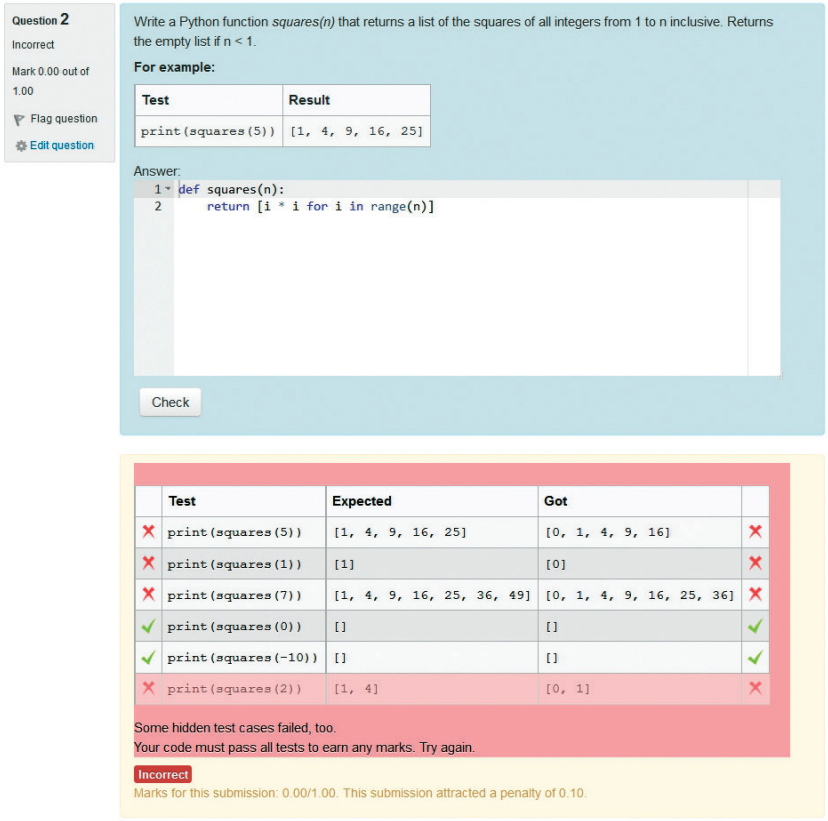
\includegraphics[scale=0.3]{pictures/CodeRunner_errada.png}
        \fonte{\cite[p.~48]{lobbharlow}}
\end{figure}

\begin{figure}[h!]
	   \centering
            \caption{CodeRunner - A simples pergunta sobre Python, respondida corretamente}
            \label{fig:ModeloConceitual}
	   	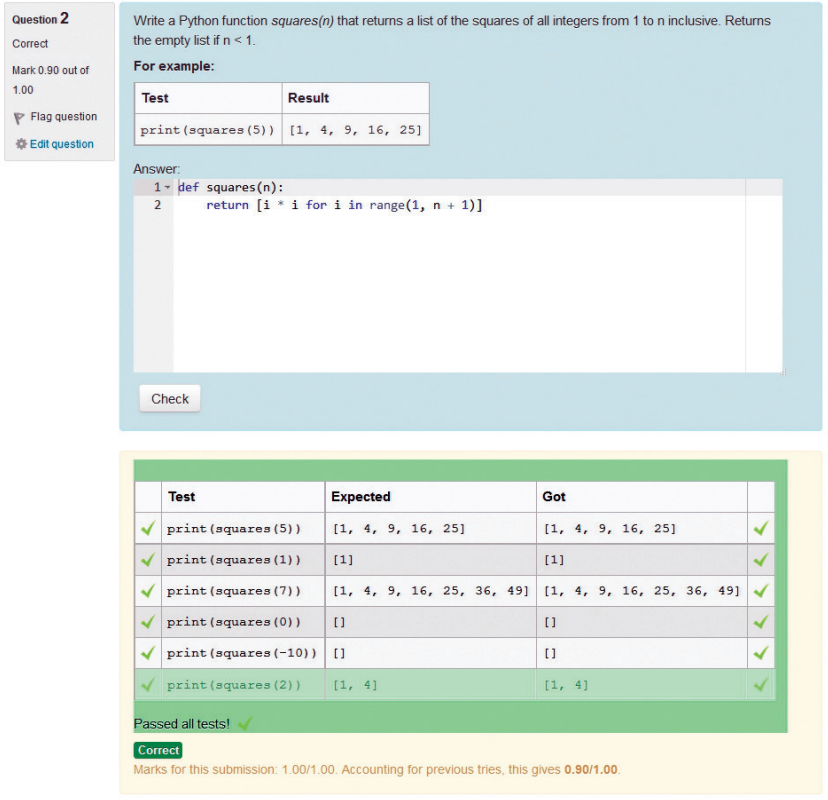
\includegraphics[scale=0.3]{pictures/CodeRunner_correta.png}
        \fonte{\cite[p.~48]{lobbharlow}}
\end{figure}

O CodeRunner possui algumas particularidades para a criação de perguntas:

\begin{enumerate} [label=(\alph*)]
    \item Cada pergunta no CodeRunner é uma instância de um protótipo de pergunta, que define o "tipo" da pergunta. Existem protótipos incorporados para perguntas comuns, como "escreva uma função", "escreva um programa" ou "escreva uma classe";
    \item Desenvolvedores de perguntas têm a liberdade de criar protótipos personalizados para oferecer funcionalidades adicionais, proporcionando uma ampla gama de possibilidades;
    \item O protótipo, por meio de um modelo, especifica o programa a ser executado para uma resposta específica do aluno, e a ser usado em caso de teste. A saída é então comparada com a saída esperada para avaliação;
    \item O uso de um modelo personalizável oferece flexibilidade ao autor da pergunta para utilizar a resposta do aluno de maneiras diversas, incluindo pré-processamentos antes da execução do código;
    \item Uma aplicação significativa dessa flexibilidade é o pré-processamento para validar submissões. Isso pode incluir a verificação de estilo usando ferramentas como pylint para Python, antes da aceitação do código para execução;
    \item O modelo também permite impor ou restringir o uso de determinadas construções de programação. Por exemplo, a reescrita do código usando um loop while em vez de um loop for pode ser obrigatória em algumas perguntas;
    \item Para garantir a segurança, a execução do código do aluno ocorre em um servidor sandbox separado, isolado do ambiente principal.
\end{enumerate}

O CodeRunner apresenta uma particularidade notável: permite que a linguagem utilizada no protótipo seja diferente daquela empregada na execução do envio do aluno. Isso é exemplificado pelo uso de um verificador de estilo local para Octave, que utiliza um modelo em Python para verificar o código antes de enviá-lo ao Octave para execução. Essa distinção entre a linguagem do modelo e o código verificado pode ser observada também, exemplificadamente, em um tipo de pergunta em que o aluno descreve uma Máquina de Estado Finito (FSM) textualmente, e o código do desenvolvedor (em Python) valida e classifica o comportamento da FSM.

A correção tradicionalmente ocorre comparando o resultado real da execução com o esperado para cada teste. No entanto, o CodeRunner possibilita incorporar o processo de classificação diretamente no modelo, como exemplificado na questão FSM. Em suma, o CodeRunner é ideal para uma ampla gama de exercícios avaliáveis por computador, oferecendo suporte a diferentes tipos de perguntas e métodos de correção.

Esse estudo mostrou um dado interessante: Realizar uma prova online em vez de uma prova escrita à mão oferece insights valiosos. O Moodle fornece estatísticas detalhadas sobre o desempenho dos alunos em cada questão, permitindo a identificação imediata de áreas temáticas que exigem mais atenção no ensino futuro, bem como questões problemáticas. A trajetória de nota de cada aluno, mostrando seu progresso durante o exame, revela padrões interessantes, como a maioria se aproximando da nota final em uma hora, enquanto alguns alunos demonstram melhora constante ao longo do tempo.

Apesar de o CodeRunner ter se revelado altamente eficaz em diversas atividades de avaliação, os autores destacaram algumas limitações fundamentais:

\begin{enumerate} [label=(\alph*)]
    \item O CodeRunner destaca-se em tarefas relativamente simples com especificações claras. Embora, teoricamente, qualquer pergunta com resposta mensurável por um programa de computador possa ser formulada como uma pergunta do CodeRunner, o esforço demandado para criar avaliadores para tarefas complexas muitas vezes inviabiliza essa abordagem, especialmente em turmas de menor tamanho;
    \item Ferramentas de qualidade de código, como o pylint, provaram ser muito valiosas para aumentar a conscientização sobre o estilo e melhorar a qualidade do código, mas ainda ocorrem abusos das regras de estilo, e a qualidade dos comentários e identificadores não pode ser avaliada por computador. Por isso, a avaliação humana ainda é reservada para a qualidade do código;
    \item A resposta a uma pergunta do CodeRunner deve ser apresentada como um único bloco de texto, predominantemente composto por código. Embora os autores das perguntas possam gerar diversos formatos de feedback, inclusive gráficos, a apresentação padrão dos resultados é tabular, com uma linha para cada caso de teste e correspondência direta entre a saída esperada e a saída real. Caso os testes exijam blocos extensos de código ou resultem em saídas volumosas, a visualização dos resultados pode dificultar a compreensão pelos alunos do motivo pelo qual uma resposta foi marcada como incorreta;
    \item A avaliação de perguntas com resultados gráficos representa um desafio. Foi criado uma simulação do kit de ferramentas GUI tkinter em Python para avaliar interfaces gráficas na disciplina, incluindo perguntas que verificam a precisão de gráficos gerados por chamadas à biblioteca de gráficos do Matlab. Contudo, a avaliação da correção de imagens ou mesmo da saída de programas que envolvem gráficos complexos, como os da biblioteca de tartarugas, foi considerada uma tarefa difícil, senão impossível;
    \item Por último, é importante ressaltar que a elaboração de perguntas de qualidade e testes eficazes pode demandar considerável tempo, mesmo em cursos de programação de nível básico. O compartilhamento de bancos de dados de perguntas entre professores seria altamente benéfico nesse contexto.
\end{enumerate}


\section{A VIRTUAL PROGRAMMING LAB FOR MOODLE WITH AUTOMATIC ASSESSMENT AND ANTI-PLAGIARISM FEATURES}

\textcite{rodriguezdelpinoandroyo} descreveram neste artigo o módulo Virtual Programming Lab (VPL) para o Moodle, desenvolvido na Universidade de Las Palmas de Gran Canaria (ULPGC), e lançado para uso gratuito sob a licença GNU/GPL.

Para empregar uma linguagem de programação específica no VPL, basta garantir que o compilador correspondente esteja devidamente instalado no sistema de execução. Atualmente, estão disponíveis sistemas de execução com instalações para diversas linguagens, incluindo Ada, C, C\+\+, C\#, FORTRAN, Haskell, Java, Octave, Pascal, Perl, PHP, Prolog, Python, Ruby, Scheme, SQL e VHDL.
 
O VPL é composto por três elementos: um módulo do Moodle, um editor de código baseado em navegador e um componente Jail, mostrados na figura 16.

\begin{figure}[h!]
	   \centering
            \caption{VPL - Componentes}
            \label{fig:ModeloConceitual}
	   	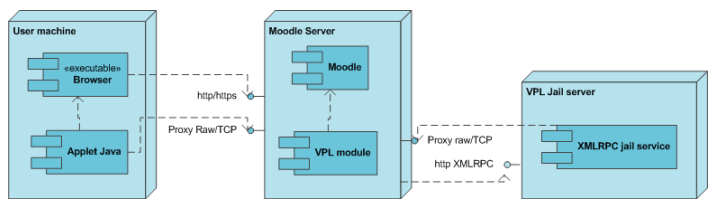
\includegraphics[scale=0.3]{pictures/VPL_componentes.png}
        \fonte{\cite[p.~2]{rodriguezdelpinoandroyo}}
\end{figure}

O VPL possui um editor de código em Java para editar, executar, depurar e avaliar programas em um ambiente simples de desenvolvimento. Para utilizar todas as funcionalidades, é necessário um navegador com suporte a JavaScript e applets Java 1.5. 

O módulo do Moodle oferece características típicas, como backup, integração com o livro de notas e controle de eventos, além de recursos específicos, como gerenciamento de submissões, suporte à avaliação e prevenção contra plágio. O módulo VPL requer Moodle 1.9.x e PHP5 ou superior. 

O componente Jail é um servidor que compila e executa códigos de alunos em um ambiente seguro, usando o comando linux chroot para restrições de leitura. Para executar ou avaliar uma submissão, é necessário ter pelo menos um servidor Jail, preferencialmente com uma distribuição Linux Ubuntu ou compatível com Red Hat. O servidor Jail atende a solicitações para execuções interativas e não interativas, com a diferença de que o segundo tipo exige dados específicos para redirecionar a entrada/saída da execução. 

Para fornecer execução no console, os servidores do Moodle precisam abrir pelo menos duas portas, sendo recomendável um número maior. Devido ao tempo prolongado para executar scripts PHP de submissões, é necessário aumentar o limite de tempo na configuração do PHP.

O módulo VPL utiliza um duplo proxy para comunicação: um lado com os clientes da Internet, atendendo às solicitações, e outro lado com os servidores Jail, executando tarefas associadas a essas solicitações. Essa abordagem possibilita diversas topologias de rede. A configuração mais simples envolve a execução do servidor Jail e do servidor Moodle no mesmo computador, embora precisem se comunicar via intranet, perdendo as vantagens de segurança do isolamento em computadores distintos. 

Uma topologia mais apropriada conecta um servidor Moodle a um ou mais servidores Jail separados, que podem estar em uma rede privada (Figura 16). Uma opção mais robusta é compartilhar vários servidores Jail entre diferentes servidores Moodle, adaptando-se a picos de carga ao alterar o número de servidores Jail usados por um servidor Moodle. A desvantagem é que os servidores Jail devem estar em um domínio público para disponibilizá-los a todos os servidores Moodle sem aumentar a complexidade da rede. 

A utilização de vários Jails não só suporta escalabilidade e melhora o desempenho, mas também oferece tolerância a falhas. Quando uma solicitação de execução é recebida pelo módulo VPL, ele escolhe aleatoriamente um servidor Jail disponível e funcional, garantindo uma resposta positiva à solicitação de disponibilidade. Se nenhum servidor for encontrado, o processo é repetido, considerando servidores que falharam anteriormente.

\begin{figure}[h!]
	   \centering
            \caption{VPL - Topologia de Rede Complexa}
            \label{fig:ModeloConceitual}
	   	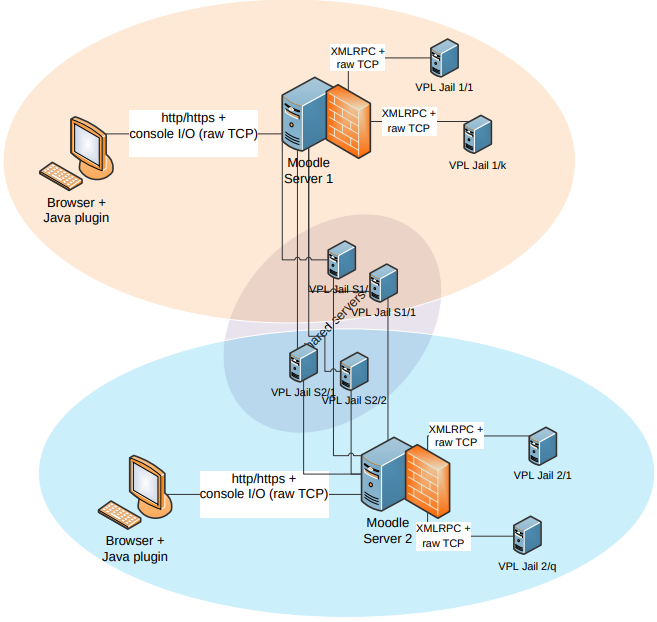
\includegraphics[scale=0.3]{pictures/VPL_topologia.png}
        \fonte{\cite[p.~2]{rodriguezdelpinoandroyo}}
\end{figure}

O VPL permite configurar, gerenciar e avaliar atividades de aprendizagem, classificadas por tipo (exemplos, exercícios de cloze, exercícios de desenvolvimento de código) e escopo (tarefas fora da sala de aula ou exames em sala).

A criação de uma atividade VPL inicia-se com o preenchimento do formulário de configuração básica no Moodle, incluindo nome, descrição, período de disponibilidade, opções de avaliação e outras configurações. Além disso, é possível especificar detalhes como número máximo de arquivos, tamanho máximo, restrições de edição, rede e senha. Veja na imagem 18.

\begin{figure}[h!]
	   \centering
            \caption{VPL - Configuração básica de restrições}
            \label{fig:ModeloConceitual}
	   	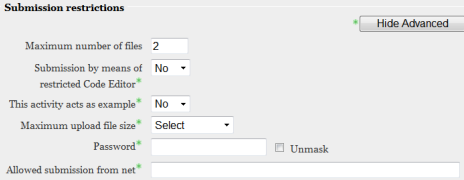
\includegraphics[scale=0.3]{pictures/VPL_config_basica.png}
        \fonte{\cite[p.~3]{rodriguezdelpinoandroyo}}
\end{figure}

Após preencher o formulário básico, o instrutor pode ajustar cinco grupos adicionais de recursos na ferramenta VPL. A guia "Descrição completa" permite fornecer detalhes sobre o problema a ser resolvido. Em "Casos de teste", é possível configurar testes com descrição, entrada, saída esperada e penalizações em caso de falha. A guia "Options" configura aspectos gerais, como a base da atividade, permissões dos alunos e se os resultados automáticos contam para a nota final. "Arquivos solicitados" determina os nomes obrigatórios dos arquivos a serem enviados. 

Essas configurações são suficientes, mas a guia "Advanced" oferece recursos adicionais para testes mais elaborados, como testes de funcionalidade avançados e outros tipos de teste, possibilitando uma avaliação abrangente da qualidade do código.

A figura 19 mostra um exemplo de configuração de casos de teste, e a figura 20 mostra a tela de configuração de casos de teste mais avançados.

\begin{figure}[h!]
	   \centering
            \caption{VPL - Exemplo de configuração de casos de teste}
            \label{fig:ModeloConceitual}
	   	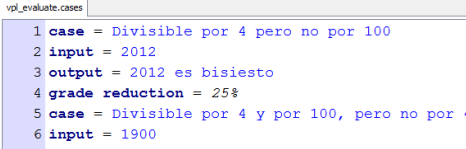
\includegraphics[scale=0.3]{pictures/VPL_testes.png}
        \fonte{\cite[p.~3]{rodriguezdelpinoandroyo}}
\end{figure}

\begin{figure}[h!]
	   \centering
            \caption{VPL - Arquivos de execução para testes avançados}
            \label{fig:ModeloConceitual}
	   	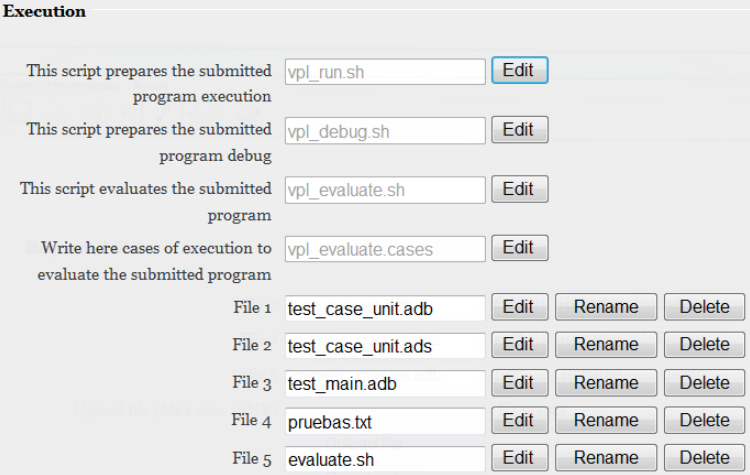
\includegraphics[scale=0.3]{pictures/VPL_testes_avancados.png}
        \fonte{\cite[p.~4]{rodriguezdelpinoandroyo}}
\end{figure}

O VPL oferece avaliação automática e assistida por computador, permitindo a personalização através das opções na guia correspondente. É essencial configurar os testes para respaldar a avaliação. O VPL realiza automaticamente os testes configurados, fornecendo um relatório com testes falhos, comentários explicativos e uma proposta de nota. O avaliador humano tem a flexibilidade de ajustar o relatório, excluindo ou adicionando comentários, reutilizando itens da lista e recalculando a nota conforme necessário.

O plágio é abordado pelo VPL através de uma ferramenta de verificação de plágio no código-fonte. Essa ferramenta procura identificar plágio entre os envios de uma tarefa em um curso, considerando também fontes como envios anteriores ou tarefas similares de outros cursos. O processo de identificação de semelhanças entre os arquivos de origem envolve três etapas: tokenização, comparação e clusterização. 

A tokenização visa obter uma assinatura normalizada para facilitar a comparação eficiente, envolvendo análise lexical, filtragem e normalização. Esse processo cria uma assinatura do programa, que é uma representação normalizada dos arquivos de código-fonte de um usuário, otimizando o processo de comparação, permitindo a detecção eficaz de plágio.

Em resumo, o Virtual Programming Lab (VPL) apresenta-se como uma ferramenta abrangente para o gerenciamento de atividades de programação. Com recursos que vão desde a configuração detalhada de atividades no Moodle até a execução de testes avançados e a detecção de plágio, o VPL oferece uma variedade de funcionalidades para apoiar a aprendizagem prática e avaliação de habilidades de programação. Destaca-se, além disso, a necessidade de configurar todos os exercícios e seus casos de teste, para disponibilização destes aos alunos.

\section{COMPARAÇÃO ENTRE OS TRABALHOS}

O estudo de \cite{cruz2022} ressalta a eficácia da integração da plataforma Beecrowd em um plano de ensino inovador para disciplinas de programação. Ao incorporar estratégias como sala de aula invertida e gamificação, a pesquisa conclui que o Beecrowd, utilizado como suporte para a gamificação, não só melhora o processo de ensino e aprendizagem, oferecendo suporte aos educadores e motivando os alunos, mas também contribui para a redução da evasão em cursos superiores de informática.

A aplicação das metodologias propostas no estudo dos autores demonstrou um impacto significativo no desempenho dos alunos ao longo do tempo na universidade dos autores, resultando em um crescimento notável e consistente nas notas. A ferramenta Beecrowd, destacada no estudo, é elogiada pela sua organização meticulosa de desafios em categorias e níveis de dificuldade, além de sua abordagem de maratona de programação, revelando-se eficaz em envolver os alunos de maneira imersiva.

Dessa forma, a tabela 1 fornece uma comparação detalhada da integração entre o Moodle e o Beecrowd, consolidada neste trabalho, com outras integrações de ferramentas ao Moodle discutidas em trabalhos relacionados. O objetivo é analisar as diversas decisões de implementação adotadas em cada projeto, proporcionando uma base para este estudo.

\begin{table}[htb]
        \IBGEtab{%
          \caption[Comparação entre quatro integrações de sistemas, que auxiliam no ensino da programação, com o Moodle: Beecrowd, BOCA, CodeRunner e VPL]{Comparação entre quatro integrações de sistemas, que auxiliam no ensino da programação, com o Moodle: Beecrowd, BOCA, CodeRunner e VPL}%
          \label{tabela-ibge}
        }{%
          \begin{tabular}{c c c c c}
          \toprule
           \textbf{Aspecto} & \textbf{Beecrowd} & \textbf{BOCA} & \textbf{VPL} & \textbf{CodeRunner} \\
          \midrule
          Possui Juiz Online	                        &  X	& X	& X	& X   \\ \midrule
          Fornece Feedback Imediato	                &  X	& X	& X	& X   \\ \midrule
          Criação Manual de Questões	                &  	& X	& X	& X   \\ \midrule
          Questões Prontas para Professores	        &  X	& 	& 	&    \\ \midrule
          Inserção Manual de Casos de Teste	        &  	& X	& X	& X   \\ \midrule
          Suporta Diversas Linguagens	                &  X	& X	& X	& X   \\ \midrule
          Pré-processamento de Submissões	        &  	& 	& 	& X   \\ \midrule
          Comentários de Testes Falhados	        &  	& 	& X	&    \\ \midrule
          Prevenção de Plágio	                        &  X	& 	& X	&    \\ 
          \bottomrule
        \end{tabular}%
        }{%
          \fonte{
              Produzido pela autora. 
          }%
        }
      \end{table}

A análise da tabela destaca o Beecrowd como notavelmente diferenciado em relação aos outros sistemas, sobretudo devido à presença de questões pré-existentes para os professores. Essa característica elimina a necessidade de cadastramento manual das questões de programação e seus respectivos testes, uma exigência presente nas plataformas BOCA, VPL e CodeRunner.

É importante destacar que a integração do presente trabalho vai ser feita por meio da criação de um Plugin. Já o BOCA e o CodeRunner são um tipo de questão do Moodle, e o VPL é um Módulo do Moodle.

Um aspecto distintivo e relevante nos sistemas BOCA, VPL e CodeRunner é a abordagem de desenvolvimento que incorpora a utilização de servidores separados para o Moodle e os sistemas juízes online. Essa estratégia visa garantir a execução independente e eficiente de cada componente, proporcionando benefícios tanto em termos de desempenho quanto de segurança.

Ao adotar servidores separados para o Moodle e os sistemas juízes online, essas plataformas buscam otimizar a distribuição de carga, evitando interferências ou sobrecargas que poderiam ocorrer se ambos compartilhassem o mesmo ambiente de execução. Isso resulta em uma operação mais estável e responsiva, melhorando a experiência do usuário e a eficácia do sistema como um todo.

Além disso, a separação de servidores contribui para a segurança do ambiente. Isolar o Moodle e os sistemas juízes online em ambientes independentes reduz os riscos de conflitos de segurança e potenciais vulnerabilidades que poderiam surgir se compartilhassem recursos ou permissões. Essa segregação promove uma abordagem mais robusta em termos de proteção de dados e integridade do sistema.

A escolha de servidores separados também permite uma escalabilidade mais eficiente, pois cada componente pode ser dimensionado de acordo com suas necessidades específicas sem afetar diretamente o desempenho do outro. Isso é particularmente crucial em ambientes acadêmicos, nos quais a demanda por plataformas como o Moodle e sistemas juízes online pode variar significativamente com base em fatores como o número de usuários e atividades acadêmicas.

Por outro lado, a prevenção contra plágio é uma característica crucial e distintiva tanto no Beecrowd quanto no VPL, destacando-se como um diferencial significativo dessas plataformas. Essa funcionalidade visa salvaguardar a integridade acadêmica, garantindo que os trabalhos submetidos pelos alunos sejam autênticos e originais.

No contexto do Beecrowd, a prevenção contra plágio pode envolver mecanismos avançados de análise de código-fonte, identificando padrões suspeitos que indicam possível cópia indevida. Além disso, o sistema pode empregar algoritmos e técnicas que comparam soluções de diferentes alunos, buscando similaridades que ultrapassem limites aceitáveis de coincidência.

No caso do VPL, a prevenção contra plágio pode ser implementada através de verificações rigorosas durante o processo de submissão. Isso pode incluir a comparação automática de códigos submetidos em busca de trechos idênticos ou substancialmente semelhantes. Além disso, o VPL pode adotar métodos de análise mais avançados, como a detecção de técnicas de programação específicas que são características de trabalhos plagiados.

Ambas as plataformas podem adotar abordagens proativas, educando os alunos sobre a importância da originalidade e as consequências éticas e acadêmicas do plágio. Isso pode incluir a disponibilização de recursos educativos sobre a elaboração de código autêntico, boas práticas de programação e a importância de citações apropriadas.

Agora sobre outros aspectos técnicos, o trabalho que relata a integração BOCA-Moodle, estudo conduzido por \cite{galasso}, traz detalhes técnicos de decisões de implementação interessantes. Os autores adotaram uma abordagem em que os dois ambientes, Moodle e BOCA, operam de forma independente. Uma característica notável é o uso do PostgreSQL como banco de dados, exigindo que o Moodle use o mesmo sistema. Assim, para que seja possível a comunicação entre banco de dados em locais distintos, foi usado o Dblink no PostgreSQL. Além disso, foram utilizadas doze tabelas no banco de dados do sistema BOCA, sendo que a integração entre o BOCA e o Moodle foi feita através da criação de gatilhos (triggers). 

Já o trabalho de \textcite{rodriguezdelpinoandroyo} traz detalhes interessantes do módulo Virtual Programming Lab (VPL). Ele possui um editor de código em Java para editar, executar, depurar e avaliar programas em um ambiente simples de desenvolvimento. Dessa forma, para utilizar todas as funcionalidades é necessário um navegador com suporte a JavaScript e applets Java. Também é composto por um componente Jail: servidor que compila e executa códigos de alunos em um ambiente seguro, usando o comando linux chroot para restrições de leitura, que possui algumas especificações de execução. 

\end{otherlanguage*}